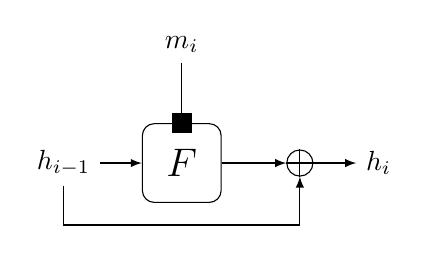
\begin{tikzpicture}
%[scale=0.7, every node/.style={scale=0.7}]

\node (f) at (0,0) [minimum size=1cm,rounded corners=1ex,draw] {\Large $F$};
\node (m) [above of=f, node distance=1.5cm] {$m_i$};
\node (h) [left of=f, node distance=1.5cm] {$h_{i-1}$};
\node (p) [right of=f, node distance=1.5cm, circle, draw] {};
\node (H) [right of=p, node distance=1cm] {$h_i$};
\draw node at (f.north) [fill,draw] {};
\draw[-] (p.north) -- (p.south);
\draw[-] (p.east) -- (p.west);
\draw[-] (m) -- (f);
\draw[-latex] (h) -- (f);
\draw[-latex] (f) -- (p);
\draw[-latex] (p) -- (H);
\draw[-latex] (h.south) -- +(0cm,-0.5cm) -|  (p.south);

\end{tikzpicture}